\newpage
{\bfseries МРНТИ 61.31.00}
\hfill {\bfseries \href{https://doi.org/10.58805/kazutb.v.2.23-443}{https://doi.org/10.58805/kazutb.v.2.23-443}}

\sectionwithauthors{К.Т. Жантасов, А.Ж.Зият, Р.Р.Якубова, М.К. Жантасов, Б.А Сакыбаев}{ИССЛЕДОВАНИЯ И РЕАЛИЗАЦИЯ ТЕХНОЛОГИИ ПОЛУЧЕНИЯ
ОРГАНОМИНЕРАЛЬНОГО УДОБРЕНИЯ -- ТУКОСМЕСИ}

\begin{center}
{\bfseries К.Т. Жантасов, А.Ж.Зият, Р.Р.Якубова, М.К. Жантасов, Б.А Сакыбаев}

Южно-Казахстанский университет им. М.Ауэзова, Шымкент, Казахстан

Корреспондент-автор: manapjan\_80@mail.ru
\end{center}

Приведены краткие сведения о проведенных НИР по получению
органоминеральных тукосмесей пролонгированного действия, содержащих
влагоудерживающие и сорбционное вещества, на основе обогащенного и
обожженного вермикулита, фосфогипса, гуматы и микроэлементы, которые
содержатся во внутренних вскрышных породах, образующихся при добыче и
подготовке бурых углей. Фосфорит, природный вермикулит, внутренние
вскрышные породы, взятые в определенных соотношениях, смешивают и
подвергают термической обработке при температуре 850--950
\textsuperscript{0}С. Полученный полупродукт охлаждают, смешивают с
бурым углем и фосфогипсом, измельчают их для повышения его
физико-химической активации. Затем к продукту добавляют 40 \% водный
раствор К\textsubscript{2}СО\textsubscript{3}, аммофос или аммиачную
селитру. Полученное сложно-смешанное удобрение перемешивают и
складируют. Получено сложно-смешанное удобрение (тукосмеси)
пролонгированного действия «ЖАМБ-70». Данное удобрение представляет
собой поликомпонентное удобрение пролонгированного действия, содержащее
азот, фосфор, калий, гумус, микроэлементы и влагоудерживающие вещества,
которое может быть использовано для известкования кислых и засоленных
почв. Предложена технологическая схема получения минерального удобрения
«ЖАМБ-70». Разработаны проектно-сметная документация, техно-рабочие
чертежи и проводятся строительно-монтажные работы по созданию
технологической линии получения минерального сложно-смешанного удобрения
пролонгированного действия «ЖАМБ-70».

{\bfseries Ключевые слова:} сложно-смешанное удобрение, фосфоритная мелочь,
фосфогипс, вермикулит, гуматы, тукосмесь пролонгированного действия,
монтаж опытно-промышленной установки

\begin{center}
{\large\bfseries ОРГАНОМИНЕРАЛДЫ ТЫҢАЙТҚЫШ - ТУКО ҚОСПАСЫН АЛУ ТЕХНОЛОГИЯСЫН ЗЕРТТЕУ ЖӘНЕ ІСКЕ АСЫРУ}

{\bfseries К.Т.Жантасов, А.Ж.Зият, Р.Р.Якубова, М.К.Жантасов, Б.А.Сакыбаев}

М.Әуезов атындағыОңтүстік Қазақстан университеті, Шымкент, Қазақстан,

e-mail: manapjan\_80@mail.ru
\end{center}

Қоңыр көмірді өндіру және дайындау кезінде пайда болатын ішкі аршу
жыныстарында кездесетін байытылған және күйдірілген вермикулит,
фосфогипс, гуматтар мен микроэлементтер негізінде құрамында ылғал
сақтайтын және сорбциялық заттар бар ұзақ әсер ететін органоминералды
тукосместерді алу бойынша жүргізілген ҒЗЖ туралы қысқаша мәліметтер
келтірілген. Фосфорит, табиғи вермикулит, белгілі бір арақатынаста
алынған ішкі аршылған жыныстар араласады және 850-950
\textsuperscript{о}С температурада термиялық өңдеуден өтеді. Алынған
жартылай өнім салқындатылады, қоңыр көмір мен фосфогипспен араласады,
оның физикалық-химиялық активтенуін арттыру үшін ұнтақталады. Содан
кейін өнімге 40\% к\textsubscript{2}со\textsubscript{3} сулы ерітіндісі,
аммофос немесе аммоний нитраты қосылады. Алынған күрделі-аралас
тыңайтқыш араластырылып, жиналады."ЖАМБ-70" ұзақ әсер ететін күрделі
аралас тыңайтқыш (қоспалар) алынды. Бұл тыңайтқыш-құрамында азот,
фосфор, калий, гумус, микроэлементтер және ылғал сақтайтын заттар бар,
қышқыл және тұзды топырақты әктеу үшін қолдануға болатын ұзақ әсер
ететін поликомпонентті тыңайтқыш."ЖАМБ-70" минералды тыңайтқышын алудың
технологиялық схемасы ұсынылды. Жобалық-сметалық құжаттама әзірленді,
техно-жұмыс сызбалары және "ЖАМБ-70"ұзақ әсер ететін минералды
күрделі-аралас тыңайтқышты алудың технологиялық желісін құру бойынша
құрылыс-монтаждау жұмыстары жүргізілуде.

{\bfseries Түйін сөздер} күрделі-араластыңайтқыш, фосфоритұсақ-түйегі,
фосфогипс, вермикулит, гуматтар, ұзақ әсер ететін тукосмесь,
тәжірибелік-өнеркәсіптік қондырғыны монтаждау

\begin{center}
{\large\bfseries RESEARCH AND IMPLEMENTATION OF TECHNOLOGY FOR PRODUCING ORGAN MINERAL FERTILIZER -- FERTILIZER MIXTURE}

{\bfseries K.T.Zhantasov, A.Zh.Ziyat, R.R.Yakubova., M.K.Zhantasov,
B.A.Sakibayev}

M.Auezov South Kazakhstan University, Shymkent, Kazakhstan,

e-mail: manapjan\_80@mail.ru
\end{center}

Brief information is provided on the research carried out on the
production of organ mineral fertilizer mixtures of prolonged action,
containing moisture-retaining and sorption substances, based on enriched
and calcined vermiculite, phosphogypsum, humates and microelements,
which are contained in internal overburden rocks formed during the
mining and preparation of brown coals. Phosphorite, natural vermiculite,
internal overburden rocks, taken in certain proportions, are mixed and
subjected to heat treatment at a temperature of 850--950
\textsuperscript{0}C. The resulting intermediate product is cooled,
mixed with brown coal and phosphogypsum, and crushed to increase its
physical and chemical activation. Then a 40 \% aqueous solution of
K\textsubscript{2}CO\textsubscript{3}, ammophos or ammonium nitrate is
added to the product. The resulting complex mixed fertilizer is mixed
and stored. A complex mixed fertilizer (fertilizer mixture) of prolonged
action ``ZHAMB-70'' was obtained. This fertilizer is a multi-component
long-acting fertilizer containing nitrogen, phosphorus, potassium,
humus, microelements and water-retaining substances, which can be used
for liming acidic and saline soils. A technological scheme for obtaining
the mineral fertilizer ``ZHAMB-70'' has been proposed. Design and
estimate documentation, technical and working drawings have been
developed, and construction and installation work is being carried out
to create a technological line for the production of mineral complex
mixed fertilizer of prolonged action ``ZHAMB-70''.

{\bfseries Keywords:} complex mixed fertilizer, phosphate rock,
phosphogypsum, vermiculite, humates, long-acting fertilizer mixture,
installation of a pilot plant.

\begin{multicols}{2}
{\bfseries Введение.} Интенсификация земледелия предполагает внедрение
новых технологий, обеспечивающих сохранение и повышение плодородия
пахотных почв, оптимальные (по условиям максимальной окупаемости
производственных ресурсов) уровни минерального питания и параметры
защиты растений, устойчивости их к стрессовым факторам.

Интенсивное использование почвенного покрова в районах земледелия
Республики Казахстан без учета агроэкологического потенциала территории
и научно-обоснованных систем земледелия, привело к значительному
снижению почвенного плодородия, деградации земель и опустыниванию, а
также развитию водной и ветровой эрозии {[}1,2{]}.

Организация полноценного и эффективного минерального питания растений
является основой производства продукции растениеводства. Дороговизна
средств химизации, исчерпаемость и невозобновляемость запасов
фосфорсодержащего сырья страны для производства удобрений, особенности
метаболизма соединений азота в растениях, почвенной и водной средах,
актуализируют проблемы наиболее эффективной технологии производства из
природных и техногенных вторичных ресурсов, применения минеральных
удобрений,а также сокращения их непроизводительных потерь.

Новизной проводимых НИР и предлагаемой технологии является получение
гуматов в почвенном покрове, за счет протекания химических реакций между
щелочными металлами натрия и калия с углеродом, входящих в состав
внутренних вскрышных пород, образовавшихся при добыче бурых углей. Кроме
этого, при получении тукосмеси, в зависимости от химического состава
почвы, где будет применяться тукосмесь, варьируется соотношение
компонентов исходных шихтовых материалов и при необходимости введение
аммофоса и серы.

В настоящее время по запасам фосфорного сырья Казахстан занимает
четвертое место в мире, имеется 4 млрд. тонн извлекаемых запасов
фосфорсодержащих руд, 15 млрд. тонн - прогнозируемых запасов. Так,
например, Каратауский бассейн фосфоритовой руды является одним из
крупнейших в мире и расположен в Жамбылской и Туркестанской областях. В
пределах Каратауского бассейна выявлено 45 месторождений фосфоритов.
Крупнейшими из них являются: Жанатасское, Кокджонское, Коксуйское,
Гиммельфарбское, Ушбасское {[}1-4{]}.

В то же время комплексные удобрения обеспечивают более эффективную и
хорошую доступность питательных веществ корневой системе. Применение
комплексных удобрений позволяет не только удовлетворить потребность
растений в питательных веществах, но и обеспечивает экономию на
транспортных расходах, строительстве складов, использовании
механизированных средств при погрузке, разгрузке и внесении удобрений в
почву {[}5-8{]}.

{\bfseries Материалы и методы.} В качестве сырьевых компонентов, при
получении органоминерального удобрения -- тукосмеси, применяются
природные и техногенные сырьевые ресурсы: отсевы природных фосфоритной,
вермикулитовой обогащенной мелочи, внутренние вскрышные породы,
образующиеся при добыче бурых углей, мелочь бурого угля, фосфогипса,
бикарбонат калия, комовая сера и аммофос {[}9-13{]}.

Технология производства органоминерального удобрения тукосмеси
представляет собой следующее. Фосфорит, природный вермикулит, внутренние
вскрышные породы, взятые в определенных соотношениях, смешивают и
подвергают термической обработке при температуре 850--950
\textsuperscript{0}С, в течение 15-20 минут. Полученный полупродукт,
содержащий Р\textsubscript{2}О\textsubscript{5} -- 16-20\%,
K\textsubscript{2}O -- 2-4\% и N -- 10-16\%, по заказу потребителя,
охлаждают, смешивают с бурым углем и фосфогипсом, измельчают их для
повышения его физико-химической активации. Затем к продукту добавляют 40
\% водный раствор К\textsubscript{2}СО\textsubscript{3}, аммофос или
аммиачную селитру. Полученное сложно-смешанное органоминеральное
удобрение перемешивают и складируют {[}10-13{]}.

Исследованиями авторов {[}14-18{]} установлена необходимость термической
активации или, так называемое термическое обогащение, при переработке
природных фосфоритов для получения органоминеральных удобрений из бедных
фосфоритных руд, которая позволяет улучшить показатели последующей
кислотной обработки, увеличивает коэффициент разложения фосфатов,
уменьшает расход серной кислоты, повышает скорость фильтрации
осаждаемого фосфогипса, снижает пенообразование и влажность фосфогипса и
т.д.

Процесс обогащения природных сырьевых материалов и в частности природных
руд делится на: термохимические, радиометрические и химические.
Химические процессы обогащения применяют в комбинированных схемах
повышения необходимого полезного компонента. К химическим методам
обогащения можно отнести гидрометаллургические, термохимические,
пирометаллургические процессы, сульфатизирующий и восстановительный
обжиг, а также другие. Наибольшее распространение в промышленности
получили гидрометаллургические процессы, которые применяют, для:

- переработки сложного по составу минерального сырья;

- доводки бедных некондиционных концентратов и других продуктов путем
удаления из них примесей;

- переработки черновых коллективных концентратов с целью полного
селективного излечения полезных компонентов.

Так, например, сернокислотное выщелачивание применяется при обогащении
природного фосфорита с последующим извлечением
Р\textsubscript{2}О\textsubscript{5} его в водный раствор и
кристаллизации сульфата кальция, в присутствии водного раствора слабой
фосфорной кислоты по нижеприведенным реакциям:

Ca\textsubscript{5}F(PO\textsubscript{4})\textsubscript{3} +
nH\textsubscript{3}PO\textsubscript{4} =
5Ca(H\textsubscript{2}PO\textsubscript{4})\textsubscript{2} +
(n-7)H\textsubscript{3}PO\textsubscript{4} + HF

На второй стадии образовавшийся
Са(Н\textsubscript{2}РО\textsubscript{4})\textsubscript{2} реагирует с
серной кислотой в присутствии с фосфорной кислотой по реакции:

Ca(H\textsubscript{2}PO\textsubscript{4})\textsubscript{2} +
2H\textsubscript{2}SO\textsubscript{4} +
mH\textsubscript{3}PO\textsubscript{4} = CaSO\textsubscript{4} +
(m+2)H\textsubscript{3}PO\textsubscript{4} + 4H\textsubscript{2}O.

Хотя механизм процесса является более сложным, особенно при смешении
растворов фосфорной и серной кислот при температурах 70--80
\textsuperscript{0}С, это позволяет получение фосфорной кислоты,
содержащей до 32 \% Р\textsubscript{2}О\textsubscript{5}.

В качестве серосодержащего компонента и нейтрализатора кислых солей
вводится фосфогипс -- отход процесса обогащения природных фосфоритов и
получения экстракционной фосфорной кислоты {[}14{]}.

Предложена технологическая схема получения органоминерального удобрения
«ЖАМБ-70», представленная на рисунке 1.
\end{multicols}

\begin{figure}[H]
	\centering
	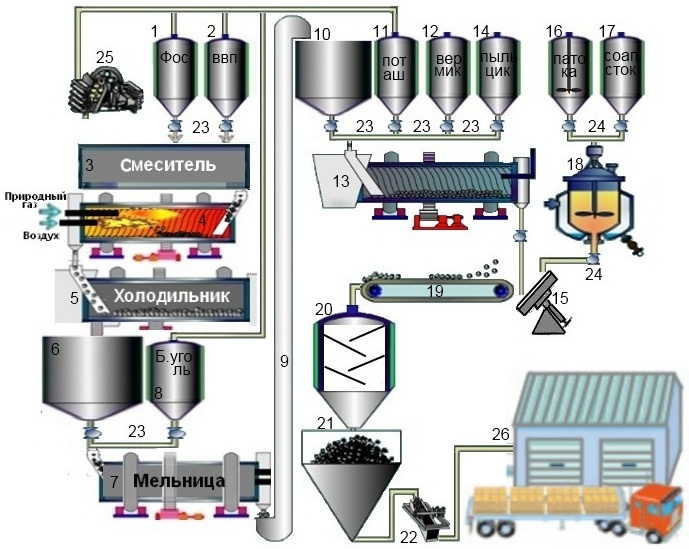
\includegraphics[width=0.75\textwidth]{assets/1081}
	\caption*{Риc.1 - Аппаратурно-технологическая схема получения органоминерального удобрения «ЖАМБ-70»}
	\caption*{1 - бункер для приема фос.сырья; 2 - бункер для приема ВВП; 3 -
смеситель двух вальный; 4 - барабанная вращавшаяся печь; 5 - холодильная
установка; 6 - бункер для приема фос.сырья; 7 - мельница шаровая; 8 -
бункер для приема бурого угля; 9 - элеватор Нори; 10 - бункер для приема
смеси фос.сырья, ВВП и бурого угля; 11 - бункер для приема поташа; 12 -
бункер для приема вермикулита; 13 - барабанный смеситель; 14 - бункер
для приема пыли циклона; 15 - ггранулятор тарельчатый; 16 - бункер для
приема патоки; 17 - бункер для приема соапстока; 18 - реактор с
мешалкой; 19 - транспортер ленточный; 20 - ступенчатый сушильный
агрегат; 21 - бункер для приема готовой продукции; 22 - фасовочная
машина; 23 - тарированные питатели; 24 - расходомер жидкости; 25 -
валковая дробилка; 26 - склад хранения продукции}
\end{figure}

\begin{multicols}{2}
{\bfseries Результаты и обсуждение.} В результате физико-химических
исследований выявлены последовательность протекающих процессов
обогащения Р\textsubscript{2}О\textsubscript{5} из природного фосфатного
сырья, за счет разложения минералов при различных температурах
{[}16-18{]}:

при 150--400 \textsuperscript{0}С -- протекает дегидратация мусковита, с
образованием парообразной воды:

KAl\textsubscript{2}{[}AlSi\textsubscript{3}O\textsubscript{10}{]}(OH)\textsubscript{2}
→ KAl\textsubscript{2}{[}AlSi\textsubscript{3}O\textsubscript{10}{]} +
H\textsubscript{2}O↑;

из октаэдрических слоев:

KMg\textsubscript{3}{[}SiAl{]}O\textsubscript{10}(OH,F)\textsubscript{2}
→
KMg\textsubscript{3}{[}SiAl{]}O\textsubscript{10}(O\textsubscript{0,5}F)\textsubscript{2}
+ H\textsubscript{2}O↑;

из глинистого минерала каолинита:

Al\textsubscript{4}(OH)\textsubscript{2}Si\textsubscript{4}O\textsubscript{10}
→ 2Al\textsubscript{2}O\textsubscript{3}*4SiO\textsubscript{2} +
4H\textsubscript{2}O↑;

при температурах 850 --900\textsuperscript{0}С протекает процесс
декарбонизации доломита, с выделением в газовую среду диоксида углерода:

CaMg(CO\textsubscript{3})\textsubscript{2} → MgO + CaCO\textsubscript{3}
+ CO\textsubscript{2}↑,

CaCO\textsubscript{3} → CaO + CO\textsubscript{2}↑;

при 750--900\textsuperscript{0}С наблюдается дегидратация
гидроксилапатита, с выделением влаги и диоксида углерода:

Ca\textsubscript{5}{[}F/(PO\textsubscript{4},CO\textsubscript{3},OH)\textsubscript{3}{]}
→
Ca\textsubscript{5}{[}F/(PO\textsubscript{4},CO\textsubscript{3},O\textsubscript{0.5})\textsubscript{3}{]}
+ 1,5H\textsubscript{2}O↑,

Ca\textsubscript{5}{[}F/(PO\textsubscript{4})\textsubscript{3}
(CO\textsubscript{3},O\textsubscript{0,5}){]} →
Ca\textsubscript{5}{[}F/(PO\textsubscript{4},O\textsubscript{1,5})\textsubscript{3}{]}
+ 3CO\textsubscript{2}↑.

На рисунке 2 представлены данные зависимости изменения содержания
различных форм Р\textsubscript{2}О\textsubscript{5} в природном
фосфорите месторождения Жанатас от температуры обжига.
\end{multicols}

\begin{figure}[H]
	\centering
	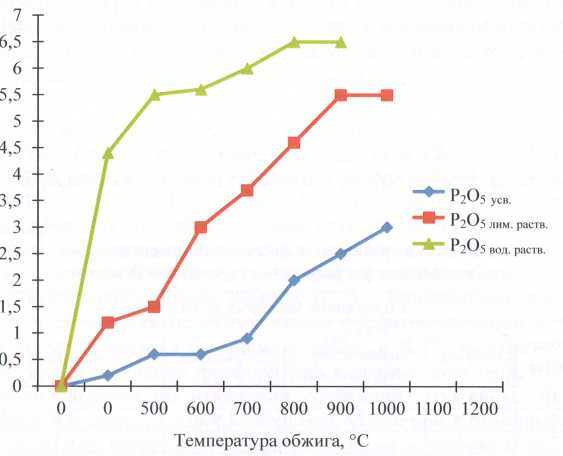
\includegraphics[width=0.45\textwidth]{assets/1082}
	\caption*{Рис. 2 - Зависимость изменения содержания различных форм Р\textsubscript{2}О\textsubscript{5} в природном фосфорите месторождения Жанатас от температуры обжига}
\end{figure}

\begin{multicols}{2}
В Белорусском технологическом университете выполнены исследования по
изучению влияние обжига на физико-химические и технологические свойства
фосфата и основных рудообразующих минералов фосфоритов {[}16{]}.
Выявлено, что в процессе обжига существенно изменяются технологические
свойства фосфоритов. Это позволяет интенсифицировать операции стадии
обогащения: измельчение, флотацию фосфоритов глауконитового типа,
сгущение и фильтрацию. Процесс обжига способствует повышению хрупкости
руды, приводит к сокращению времени тонкого измельчения и улучшает
гранулометрический состав продуктов помола {[}17{]}.

Данное удобрение представляет собой поликомпонентное удобрение
пролонгированного действия, содержащее азот, фосфор, калий, гумус,
микроэлементы и влагоудерживающие вещества, которое может быть
использовано для известкования кислых и засоленных почв. Удобрение
«ЖАМБ-70» применено на полях хозяйства «Жантас» в 2018 году, а также в
теплицах и полях хозяйства «Алтынай» в 2021 году, позволившие повысить
съем овощной сельхоз продукции в зависимости от вида культуры от 15 до
35 \% и снизить расход воды на полив до 15\%, за счет увеличения срока
между поливами на 1,5--2 суток.

Проведены испытания поликомпонентных органоминеральных удобрений на
опытных участках черноземных почв Белорусского Государственного
технологического университета Республики Беларусь, при выращивание
бобово-злаковой смеси, а также с определением его качественных
показателей на сероземных оптимальных посевных площадях КазНИИ
почвоведения и агрохимии Республики Казахстан расположенного в
Мактааральском районе Южно-Казахстанской области, при выращивании
хлопчатника с использованием рекомендации Б.Д. Доспехова, которые
позволили получить экологически чистые продукты сельскохозяйственных
культур {[}19,20{]}.

{\bfseries Выводы.} На основании проведенных исследования по получению
гранулированных комплексных удобрений на основе отходов различных
производств, содержащих влагоудерживающее и нейтрализующие вещества, а
также гуматсодержащие отходы угледобывающей промышленности, в частности
бурых углей, получено сложно-смешанное органоминеральное удобрение
(тукосмеси) пролонгированного действия «ЖАМБ-70».

В результате проведенной научной и научно-технической деятельности
(РННТД) получен грант на коммерциализацию данной научной разработки.
Разработана проектно-сметная документацияи стандарт организации СТ
2425--1958-01-ГП-002-2014 на сложно-смешанное минеральное удобрение
пролонгированного действия «ЖАМБ-70», разовый технологический регламент
производства, приобретены сырье и вспомогательные материалы, а также
оборудование для мини-цеха производительностью 2-3 тонны в час
тукосмеси.

В настоящее время разработаны проектно-сметная документация,
техно-рабочие чертежи и проводятся строительно-монтажные работы по
созданию технологической линии получения органоминерального
сложно-смешанного удобрения пролонгированного действия «ЖАМБ-70».
\end{multicols}

\begin{center}
{\bfseries Литература}
\end{center}

\begin{noparindent}
1. Лареншин В.Г., Шуравилан А.В. пути снижения деградации и современные
технологии повышения плодородия почв в антропогенных ландшафтах,
субтропической и тропической зон. Учеб. пособие - М.: РУДН. 2008. -263
с.

2. Жантасов К.Т., Айбалаева Қ.Д., Франгулиди Л.Х и др. Технологическое
оснащение производства желтого фосфора. Учебник.- Алматы, Изд. «Эверо»,
2014. -444 с

3. ЖантасовК.Т., ИскандировМ.З., Айбалаева К.Д. и др. Современные
технологии переработки минерального сырья, учебник /под ред. д.т.н,
проф. Жантасова К.Т.- Шымкент:Изд. «Элем», 2015.- 476 с.

4. Жантасов К.Т., Искандиров М.З., АйбалаеваК.Д. и др. Технология добычи
и обогащения фосфатно-кремнистого сырья Каратау, монография /под ред.
д.т.н, проф. Жантасова К.Т.-Тараз:Изд. ТОО«Рысбаев и Ко», 2016.-330 с.

5. Бишимбаев В.К., Жантасов К.Т., Дормешкин О.Б., Бажирова К.Н.
Переработка фосфоритной мелочи в сложно-смешанные минеральные удобрения
пролонгированного действия. /Труды Междунар. научно-практ. конф.
«Ауэзовские чтения--12». Т.1. - Шымкент, 2014. - С. 23-26.

6. Жантасов К.Т., Молдабеков Ш.М., Бишимбаев В.К. и др.
Индустриально-инновационная технология получения механоактивированных
сложно-смешанных поликомпонентных минеральных удобрений
пролонгированного действия. / Труды Междунар. научно-практ. конф.
«Развитие науки, образования и культуры независимого Казахстана в
условиях глобальных вызовов современности». -- Шымкент, 2013. - С.69-72.

7. Sh.Moldaberov, K.Zhantasov, O.Balabekov, O.Koblanova, M.Yeskendirova,
D.Zhantasova, K.Bazhirova,

M.Zhantasov. Own Coal Oxidation Nitric Acid
with the Nitrogen-Humic Fertilizers Production // European International
of Science and Technology -Vol.2(4), 2013.- P.41-52.

8. Отчет заключительный по теме: «Создание технологии и разработка
научных основ синтеза поликомпонентных минеральных удобрений со
специфическими особенностями для сероземных почв» № гос. регистрации
0112РК02590 / Научный руководитель д.т.н., профессор Жантасов
К.Т.-Шымкент:ЮКУ

им.М.Ауэзова, 2014.- 241 с.

9. Патент РК №27551 Способ получения сложно-смешанного минерального
удобрения. Опубл. 15.10.2013, бюл. 310.

10. Евразийский патент № 02417 Способ получения комплексного
органоминерального удобрения. Дата публикации и выдачи патента
30.06.2016.

11. Патент РК №33805 Способ получения комплексного удобрения. Опубл.
02.08.2019, бюл. №31.

12. Евразийский патент № 043932 Способ получения комплексного
органоминерального удобрения- тукосмеси. Дата публикации и выдачи патента
07.07.2023.

13. Новые виды фосфорсодержащих комплексных удобрений и тукосмесей.
Технология получения и агрохимическая эффективность: Монография/ К.Т.
Жантасов и др.: науч, ред.: О.Б. Дормешкин, К.Т. Жантасов.-- Минск.:
БГТУ, 2020 - 326 с.

14.K.Zhantasov, A. Ziyat, N. Sarypbekova, M.Zhantasov, G. Iztleuov
Ecologically friendly, slow-release granular fertilizers with
phosphogypsum. Polish Journal of Environmental Studies\emph{.-} 2020.-
31(3). - P.2935 -2942, 2020. DOI: 10.15244/pjoes/144099

15. Жантасов, К.Т. Разработка и внедрение малоотходной и
энергосберегающей технологии в производстве фосфора: Автореф. дис. д-ра
техн. наук. / К. Т. Жантасов.- Шымкент, 1998.- 45 с.

16. Бажирова К.Н. Разработка энергосберегающей технологии производства
механоактивированных комплексных минеральных удобрений пролонгированного
действия. Дисс. на соис. уч.степ. док.фил. (PhD) 6D072000 -Химическая
технология неорганических веществ. Шымкент, 2015.- 155с.

17. Байжанова С.Б. Разработка технологии получения и очистки
экстракционной фосфорной кислоты из агломерированного
фосфатно-кремнистого сырья. Дисс. на соис. уч.степ. к.т.н. по
специальности -- Технология неорганических веществ. Шымкент, 2002. -
102с.

18. Шаймерденова Г. Шартқа сәйкессіз Жаңатас кенорнының фосфатты
шикізатынан диамонийфосфат алу технологиясын әзірлеу. Дисс. на соис.
уч.степ. док.фил. (PhD) 6D072000 -- Химическая технология неорганических
веществ. Шымкент, 2022. - 131с.

19. Kamshat Bazhirova, Kurmanbek Zhantasov, Tynlybek Bazhirov, Alexandr
Kolesnikov, Zarina Toltebaeva and Nurlybek Bazhirov 1 Acid-Free
Processing of Phosphorite Ore Fines into Composite Fertilizers Using the
Mechanochemical Activation Method. J. Compos. Sci. 2024, 8, 165.
https://doi.org/10.3390/jcs8050165

20. Отчет заключительный по теме: «Исследование изменения содержания
санитарно-эпидемиологических, токсикологических и радиологических
соединений в томатах, моркови, кукурузе и сое-бобовых культурах при
применении гуматосодержащих сложно-смешанных NPK-удобрений
пролонгированного действия, для обеспечения экологической безопасности»
№ гос. регистрации 0115РК01485 / Научный руководитель д.т.н., профессор
Жантасов К.Т. -- Шымкент: ЮКУ им. М.Ауэзова, 2015-2017. -- 42 с.
\end{noparindent}

\begin{center}
{\bfseries Referenses}
\end{center}

\begin{noparindent}
1. Larenshin V.G., Shuravilan A.V. Puti snizhenija degradacii i
sovremennye tehnologii povyshenija plodorodija pochv v antropogennyh
landshaftah, subtropicheskoj i tropicheskoj zon. Ucheb. Posobie- M.:
RUDN. 2008.-263 s. {[}in Russian{]}

2. Zhantasov K.T., Ajbalaeva Қ.D., Frangulidi L.H i dr. Tehnologicheskoe
osnashhenie proizvodstva zheltogo fosfora. Uchebnik. -Almaty, Izd.
«Jevero», 2014.- 444 s. {[}in Russian{]}

3. ZhantasovK.T., IskandirovM.Z., Ajbalaeva K.D. i dr. Sovremennye
tehnologii pererabotki mineral\textquotesingle nogo
syr\textquotesingle ja, uchebnik /pod red. d.t.n, prof. Zhantasova
K.T.-Shymkent:Izd. «Jelem», 2015.- 476 s. {[}in Russian{]}

4. Zhantasov K.T., Iskandirov M.Z., AjbalaevaK.D. i dr. Tehnologija
dobychi i obogashhenija fosfatno-kremnistogo syr\textquotesingle ja
Karatau, monografija /pod red. d.t.n, prof. Zhantasova K.T.-Taraz:Izd.
TOO«Rysbaev i Ko», 2016.- 330 s. {[}in Russian{]}

5. Bishimbaev V.K., Zhantasov K.T., Dormeshkin O.B., Bazhirova K.N.
Pererabotka fosforitnoj melochi v slozhno-smeshannye
mineral\textquotesingle nye udobrenija prolongirovannogo dejstvija.
/Trudy Mezhdunar. nauchno-prakt. konf. «Aujezovskie chtenija--12».
T.1.-Shymkent, 2014.-S. 23-26. {[}in Russian{]}

6. Zhantasov K.T., Moldabekov Sh.M., Bishimbaev V.K. i dr.
Industrial\textquotesingle no-innovacionnaja tehnologija poluchenija
mehanoaktivirovannyh slozhno-smeshannyh polikomponentnyh
mineral\textquotesingle nyh udobrenij prolongirovannogo dejstvija. /
Trudy Mezhdunar. nauchno-prakt. konf. «Razvitie nauki, obrazovanija i
kul\textquotesingle tury nezavisimogo Kazahstana v uslovijah
global\textquotesingle nyh vyzovov sovremennosti». -- Shymkent, 2013. -
S.69 -72. {[}in Russian{]}

7. Sh.Moldaberov, K.Zhantasov, O.Balabekov, O.Koblanova, M.Yeskendirova,
D.Zhantasova, K.Bazhirova,

M.Zhantasov. Own Coal Oxidation Nitric Acid
with the Nitrogen-Humic Fertilizers Production // European International
of Science and Technology -Vol.2(4), 2013.- P.41-52.

8. Otchet zakljuchitel\textquotesingle nyj po teme: «Sozdanie tehnologii
i razrabotka nauchnyh osnov sinteza polikomponentnyh
mineral\textquotesingle nyh udobrenij so specificheskimi osobennostjami
dlja serozemnyh pochv» № gos. registracii 0112RK02590 / Nauchnyj
rukovoditel\textquotesingle{} d.t.n., professor Zhantasov
K.T.-Shymkent:JuKU im.M.Aujezova, 2014.- 241 s. {[}in Russian{]}

9. Patent RK №27551 Sposob poluchenija slozhno-smeshannogo
mineral\textquotesingle nogo udobrenija. Opubl. 15.10.2013, bjul. 310.
{[}in Russian{]}

10. Evrazijskij patent № 02417 Sposob poluchenija kompleksnogo
organomineral\textquotesingle nogo udobrenija. Data publikacii i vydachi
patenta 30.06.2016. {[}in Russian{]}

11. Patent RK №33805 Sposob poluchenija kompleksnogo udobrenija. Opubl.
02.08.2019, bjul. № 31. {[}in Russian{]}

12. Evrazijskij patent № 043932 Sposob poluchenija kompleksnogo
organomineral\textquotesingle nogo udobrenija-tukosmesi. Data publikacii
i vydachi patenta 07.07.2023. {[}in Russian{]}

13. Novye vidy fosforsoderzhashhih kompleksnyh udobrenij i tukosmesej.
Tehnologija poluchenija i agrohimicheskaja
jeffektivnost\textquotesingle: Monografija/ K.T. Zhantasov i dr.: nauch,
red.: O.B. Dormeshkin, K.T. Zhantasov.-- Minsk.: BGTU, 2020 - 326 s.
{[}in Russian{]}

14.K.Zhantasov, A. Ziyat, N. Sarypbekova, M.Zhantasov, G. Iztleuov
Ecologically friendly, slow-release granular fertilizers with
phosphogypsum. Polish Journal of Environmental Studies\emph{.-} 2020.-
31(3). - P.2935 -2942, 2020. DOI: 10.15244/pjoes/144099

15. Zhantasov, K.T. Razrabotka i vnedrenie maloothodnoj i
jenergosberegajushhej tehnologii v proizvodstve fosfora: Avtoref. dis.
d-ra tehn. nauk. / K. T. Zhantasov.- Shymkent, 1998.- 45 s. {[}in
Russian{]}

16. Bazhirova K.N. Razrabotka jenergosberegajushhej tehnologii
proizvodstva mehanoaktivirovannyh kompleksnyh
mineral\textquotesingle nyh udobrenij prolongirovannogo dejstvija. Diss.
na sois. uch.step. dok.fil. (PhD) 6D072000 -Himicheskaja tehnologija
neorganicheskih veshhestv. Shymkent, 2015.- 155s. {[}in Russian{]}

17. Bajzhanova S.B. Razrabotka tehnologii poluchenija i ochistki
jekstrakcionnoj fosfornoj kisloty iz

aglomerirovannogo
fosfatno-kremnistogo syr\textquotesingle ja. Diss. na sois. uch.step.
k.t.n. po special\textquotesingle nosti -- Tehnologija neorganicheskih
veshhestv. Shymkent, 2002. - 102s. {[}in Russian{]}

18.Shajmerdenova G. Shartқa sәjkessіz Zhaңatas kenornynyң fosfatty
shikіzatynan diamonijfosfat alu tehnologijasyn әzіrleu. Diss. na sois.
uch.step. dok.fil. (PhD) 6D072000 -- Himicheskaja tehnologija
neorganicheskih veshhestv. Shymkent, 2022. - 131s. {[}in Kazakh.{]}

19. Kamshat Bazhirova, Kurmanbek Zhantasov, Tynlybek Bazhirov, Alexandr
Kolesnikov, Zarina Toltebaeva and Nurlybek Bazhirov 1 Acid-Free
Processing of Phosphorite Ore Fines into Composite Fertilizers Using the
Mechanochemical Activation Method. J. Compos. Sci. 2024.-Vol. 8(5).-
P.165. https://doi.org/10.3390/jcs8050165

20. Otchet zakljuchitel\textquotesingle nyj po teme: «Issledovanie
izmenenija soderzhanija sanitarno-jepidemiologicheskih,

toksikologicheskih i radiologicheskih soedinenij v tomatah, morkovi,
kukuruze i soe-bobovyh kul\textquotesingle turah pri primenenii
gumatosoderzhashhih slozhno-smeshannyh NPK-udobrenij prolongirovannogo
dejstvija, dlja obespechenija

jekologicheskoj bezopasnosti» № gos.
registracii 0115RK01485 / Nauchnyj rukovoditel\textquotesingle{} d.t.n.,
professor Zhantasov K.T. -- Shymkent: JuKU im. M.Aujezova, 2015-2017. -
42.{[}in Russian{]}
\end{noparindent}

\emph{{\bfseries Сведения об авторах}}

\begin{noparindent}
Жантасов К.Т. {\bfseries --} доктор технических наук, профессор, заведующий
научно-исследовательской лаборатории, Южно-Казахстанский университет им.
М.Ауэзова, Шымкент, e-mail: k\_zhantasov@mail.ru;

Зият А.Ж. -- преподаватель, Южно-Казахстанский университет им.
М.Ауэзова, Шымкент, e-mail:ziyat.a@mail.ru;

Якубова Р.Р. - кандидат технических наук, доцеент, Южно-Казахстанский
университет им. М.Ауэзова, Шымкент, e-mail:yarr-57@mail.ru

Жантасов М.К. {\bfseries --} кандидат технических наук, ассоциированный
профессор, заведующий кафедрой, Южно-Казахстанский университет им.
М.Ауэзова, Шымкент, e-mail: manapjan\_80@mail.ru;

Сакыбаев Б.А. -- PhD, ст. преподаватель, Южно-Казахстанский университет
им. М.Ауэзова, Шымкент, e-mail:neftehimstroy@mail.ru
\end{noparindent}

\emph{{\bfseries Information about the authors}}

\begin{noparindent}
Zhantasov K.T. - Doctor of Technical Sciences, Professor, Head of the
Laboratory. M.Auezov South Kazakhstan University, Shymkent, e-mail: :
k\_zhantasov@mail.ru;

ZiyatA.Zh. -- teacher, M.Auezov South Kazakhstan University, Shymkent,
e-mail:ziyat.a@mail.ru;

Yakubova R.R. - Candidate of Technical Sciences, Associate
Professor,M.Auezov South Kazakhstan University, Shymkent, e-mail:
yarr-57@mail.ru;

Zhantasov M.K. - Candidate of Technical Sciences, Associate Professor,
Head of the Department. M.Auezov South Kazakhstan University, Shymkent,
e-mail: manapjan\_80@mail.ru;

Sakybayev B.A. - PhD, teacher, M.Auezov South Kazakhstan University,
Shymkent, e-mail:neftehimstroy@mail.ru
\end{noparindent}
